\documentclass[10pt]{beamer}
\usetheme{Copenhagen}

\usepackage{comment}

\usepackage[backend=biber, style=alphabetic, sorting=none, bibstyle=alphabetic, maxnames=10, minnames=6,backref=true, autocite=inline, labelalpha=true, doi=false, url=false]{biblatex}
\addbibresource{the.bib}

\usepackage{tikz}
\usetikzlibrary{arrows.meta, positioning}

\usepackage{graphicx}
\graphicspath{ {./images/} }

\title[Parametrizando un Sistema Informático para Obra Social Universitaria]
{Parametrizando un Sistema Informático para Obra Social Universitaria con un Motor de Reglas}
\author{Iván Brocas}

\begin{document}

\maketitle
\begin{comment}
(Presentación mía y del trabajo)
\end{comment}

\section{Introducción}

\begin{frame}{Introducción}{Marco de trabajo}
    Un sistema informático para obras sociales universitarias, caracterizado por:
    \begin{itemize}
        \item Ágilidad
        \item Centricidad en el afiliado
    \end{itemize}
    % TODO: Tecnologías
\end{frame}
\begin{comment}
Este projecto se encuentra enmarcado en el desarrollo de un sistema informático para obras sociales universitarias, caracterizado por:
- Ágilidad
- Centricidad en el afiliado
El foco se encuentra en la segunda, procurando facilitar la adaptación del sistema en respuesta a cambios a un costo accesible y en tiempos mínimos a partir de la introducción de un motor de reglas que permita separar el código fuente de reglas del negocio tendientes a cambiar.
\end{comment}

\subsection{Motivación}

\begin{frame}{Motivación}
    \begin{itemize}
        \item El contexto de las obras sociales universitarias está en constante cambio
        \item Un sistema que falla en adaptarse pierde su utilidad:
        \begin{itemize}
            \item Aumento en el trabajo del personal
            \item Disminución en la calidad de los servicios
            \item Menos información para la toma de decisiones
        \end{itemize}
    \end{itemize}
\end{frame}
\begin{comment}
La motivación de este trabajo parte, principalmente, de dos observaciones
- El contexto de las obras sociales universitarias está en constante cambio
- Un sistema que falla en adaptarse pierde su utilidad, en la medida en que las funcionalidades brindadas por el mismo no son adaptadas para acomodar los cambios en el contexto. Esta perdida de utilidad suele manifestarse en forma de
    - Aumento en el trabajo del personal: el cual tiene que responder para tener en cuenta los cambios que el sistema no tuvo. Este trabajo manual además reemplaza parte del trabajo que estaba previamente automatizado.
    - Disminución en la calidad de servicio: El aumento en la porción del trabajo manual se traduce en un aumento de los tiempos necesarios para llevar a cabo trámites y tareas dentro de la obra social, lo que resulta en la pérdida de la calidad percibida por los afiliados.
    - Menos información para la toma de decisiones: La disminución en la porción del trabajo automatizado conlleva una disminución correspondiente en la capacidad del sistema para recolectar información, con la cual respaldar la toma de decisiones.
\end{comment}

\begin{frame}{Posibles soluciones}
    \begin{itemize}
        \item Incorporar/escalar su propia área de informática de manera que esté a la altura del desarrollo y mantenimiento de software necesarios
        \item Contratar a una empresa para que esté a cargo de este desarrollo y mantenimiento
        \item Comprarle a una empresa el producto ya desarrollado y pagar por su adaptación y mantenimiento
    \end{itemize}
\end{frame}
\begin{comment}
Las soluciones a las que pueden recurrir las obras sociales universitarias para reducir la indicidencia de estos problemas pueden clasificarse de forma general en
- incorporar/escalar su propia área de informática de manera que esté a la altura del desarrollo y mantenimiento de software necesarios
- contratar a una empresa para que esté a cargo de este desarrollo y mantenimiento
- comprarle a una empresa el producto ya desarrollado y pagar por su adaptación y mantenimiento

Las primeras dos opciones requieren que la obra social sea propietaria del sistema en cuestión.

Por otra parte, la última opción, en principio parece ser más onerosa y rápida de concretar. Sin embargo, un mayor poder de desición por parte de los afiliados, junto con un menor tamaño de la obra social, el cual suele implicar mayor complejidad en los convenios con proveedores, resultan en una mayor complejidad en comparación con su contraparte privada. Esta complejidad adicional necesariamente incrementa los costos de adaptación y mantenimiento, reduciendo la atractividad de está opción en un contexto de recursos limitados.
\end{comment}

\subsection{Objetivos}

\begin{frame}{Objetivos}
    \begin{block}{Objetivo General}
        Facilitar la adaptación del sistema frente a cambios en la reglamentación del cálculo de cuotas.
    \end{block}
    \begin{block}{Objetivos Específicos}
        \begin{enumerate}
            \item Extraer las reglas de negocio actualmente en uso
            \item Expresar dichas reglas en un lenguaje que resulte entendible para el personal de la obra social.
            \item Permitir la gestión de las especificaciones obtenidas de forma independiente al sistema.
            \item Reducir el esfuerzo requerido para materializar cambios en las reglas del negocio
            \begin{enumerate}
                \item modificar el código fuente del sistema, ni
                \item realizar el despliegue de una nueva versión.
            \end{enumerate}
            \item Reformular el código fuente para que sea más legible.
        \end{enumerate}
    \end{block}
\end{frame}
% TODO: agregar métrica
\begin{comment}
El principal objetivo es facilitar la adaptación del sistema frente a cambios en su contexto. En particular, se focaliza en el cálculo de cuotas de los afiliados. Se eligió esta parte de las reglas de negocio en concreto por su complejidad y propensidad a cambios.
Una forma de lograr esto es mediante la separación de las reglas de negocio del código fuente. Para esto, se suele hacer uso de un motor de reglas, que permite la ejecución de reglas externas al código de la aplicación. Este motor suele formar parte de un sistema de gestión de reglas de negocio, que además del motor incluye herramientas para la gestión de las reglas.

De este objetivo se extraen los objetivos específicos

- Extraer las reglas de negocio actualmente en uso, partiendo de la documentación correspondiente y la materialización de las reglas de negocio presente en el código fuente. Las reglamentaciones utilizadas son las que se encontraban en vigor durante la última actualización del código fuente (documento de 2023).
- Expresar dichas reglas en un lenguaje que resulte entendible para el personal de la obra social.
- Permitir la gestión de las especificaciones obtenidas de forma independiente al sistema.
- Reducir el esfuerzo requerido para materializar cambios en las reglas del negocio
    - modificar el código fuente del sistema, ni
    - realizar el despliegue de una nueva versión.

Se espera que el logro de estos objetivos reduzca o elimine la incidencia de los problemas antes mencionados

Por otro lado, partiendo de la revisión de la implementación actual de las reglas de negocio en el código fuente, se agrega un objetivo adicional:
- Reformular el código fuente para que sea más legible.

Esto para mejorar la compresión de la implementación actual y brindar un mejor punto de partida para la posterior comparación con el motor de reglas.
\end{comment}

\section{Revisión literaria}

\subsection{Trabajos Relacionados}
\begin{frame}{Revisión literaria}{Trabajos Relacionados}
    \begin{itemize}
        \item Calculation of Insurance Policy Prices Using Rules-based Systems\footfullcite{medic2019calculation}
        \item Un sistema operacional mejorado con el uso de un motor de reglas de negocio. El caso SENASA\footfullcite{sampol2019sistema}
    \end{itemize}
\end{frame}
\begin{comment}
Para cumplir con los objetivos propuestos, se comenzó por realizar una revisión de la literatura disponible afín al tema. Primeramente, se realizó la búsqueda de trabajos similares, los trabajos de mayor similitud fueron:

En el primer trabajo se reporta un uso similar de un BRMS para el cálculo de los precios de las distintas pólizas de una aseguradora, siendo el principal objetivo buscado la mantenibilidad y la adaptabilidad a cambios en las regulaciones.

El segundo trabajo, en el contexto nacional, se describe el uso de un BRMS en aplicaciones desarrolladas para SENASA con el objetivo de lograr que tengan mayor flexibilidad frente a cambios en las reglas de negocio que rigen los proceso que soportan.

También se detectó que en sistemas informáticos para organismos de salud privados, se argumenta flexibilidad en la especificación de reglas de negocio, pero sin mayor detalle que el comercial.
\end{comment}

\subsection{Afiliaciones y cálculo de cuotas}

\begin{frame}{Afiliaciones y cálculo de cuotas}
    En DOSPU se dividen a los afiliados en las categorías:
    \begin{itemize}
        \item Titular
        \item Familiar
        \item Voluntario adherente
    \end{itemize}
    % TODO: agregar referencias
\end{frame}
\begin{comment}
De las ordenanzas que dictan las normativas de DOSPU, podemos ver que los afiliados estan divididos en tres subcategorías:
- Titular
- Familiar, de un afiliado titular
- Voluntario Adherente
\end{comment}

\begin{frame}{Titular}
    \begin{block}{Obligatorio activo}
        Actualmente no calculado de forma directa por el sistema
    \end{block}
    \begin{block}{Voluntario jubilado}
        Monto de la cuota:
        \begin{displaymath}
        0.02 * j_m + 0.05 * j_h
        \end{displaymath}

        , donde:
        \begin{itemize}
            \item $j_m = \text{jubilación mínima}$
            \item $j_h = \text{haber jubilatorio}$
        \end{itemize}
    \end{block}
\end{frame}
\begin{comment}
Los titulares, a su vez, se dividen en:
- Obligatorio activo: agentes que se encuentren en actividad, como docentes, por ejemplos.
    Actualmente, no calculado de forma directa por el sistema, con lo cual queda fuera del alcance de este trabajo.
- Jubilados voluntarios: previamente obligatorios activos que optan por continuar estando afiliados.
Su cuota está calculada por la fórmula (fórmula en la diapositiva.)

Dos consideraciones adicionales que se extrajeron del código fuente del sistema, es que en caso de que dos afiliados voluntarios jubilados tengan registrado un vínculo de cónyuge, se aplica un descuento de 30% a la cuota del afiliado con menor haber jubilatorio. Para esto, ambos afiliados deben tener registrado un haber jubilatorio.

En caso de no tener un haber jubilatorio, en lugar de utilizarse la fórmula mostrada, se utiliza valor de referencia
\end{comment}

\begin{frame}{Familiar}
    \begin{block}{Familiar de obligatorio activo}
        Es no aportante
    \end{block}
    \begin{block}{Cónyuge o conviviente de voluntario jubilado}
        Monto de cuota:  70 \% de la del afiliado titular.
    \end{block}
\end{frame}
\begin{comment}
Como se mencionó antes, los afiliados de esta categoría son familiares de afiliados titulares, distinguiéndose entre
- Familiar de obligatorio activo: son no aportantes, es decir que su cuota es 0.
- Cónyuge o conviviente de voluntario jubilado: su cuota es (fórmula en la slide).
\end{comment}

\begin{frame}{Voluntario adherente}
    Subcategorías:
    \begin{itemize}
        \item pensionado
        \item becarios y personal ad honorem de la UNSL
        \item agente UNSL con licencia
        \item ascendientes en primer grado del afiliado titular
        \item hijos (que hayan dejado de reunir las condiciones de no aportantes)
        \item familiares adherentes
        \item universitarios adherentes
        \item ex-afiliados a DOSPU
        \item agentes vinculados a DOSPU
        \item adherente de edad avanzada
    \end{itemize}
\end{frame}
\begin{comment}
Como su nombre lo indica son aquellos que optan voluntariamente por ser afiliados de la obra social, pagando aportes dependientes de la subcategoría a la que pertenezcan.
Dentro de esta se esta categoría, se encuentran las siguientes subcategorías:
- pensionado
- becarios y personal ad honorem de la UNSL
- agente UNSL con licencia
- ascendientes en primer grado del afiliado titular
- hijos que hayan dejado de reunir las condiciones de no aportantes
- familiares adherentes
- universitarios adherentes
- ex-afiliados a DOSPU
- agentes vinculados a DOSPU
- adherente de edad avanzada
\end{comment}

\begin{frame}{Voluntario adherente}
    \begin{block}{Caso general}
        Porcentaje sobre la Cuota Mensual Máxima Única (CMMU), dependiente de la edad.

        CMMU: 6 \% del sueldo total bruto de un Profesor Universitario Titular Exclusivo con Máxima Antigüedad
    \end{block}
    \begin{block}{Pensionado}
        Monto de la cuota:
        \begin{displaymath}
        0.02 * j_m + 0.05 * p
        \end{displaymath}

        , donde:
        \begin{itemize}
            \item $j_m = \text{jubilación mínima}$
            \item $p = \text{pensión}$
        \end{itemize}
    \end{block}
\end{frame}
\begin{comment}
En general, el monto a pagar por los afilaidos voluntarios adherente se calcula como un porcentaje sobre la Cuota Mensual Máxima Única (CMMU) (definición en la slide). Este porcentaje es dependiente de la edad del afiliado.

Para algunas de las subcategorías se utiliza otra fórmula, o se tienen consideraciones adicionales. Estas excepciones se presentan a continuación.

El cálculo para un pensionado sigue casi las mismas consideraciones que el cálculo de un voluntario jubilado, con la excepción del descuento aplicado para los afiliados de la misma categoría con vínculo por cónyuge.
\end{comment}

\begin{frame}{Voluntario adherente}
    \begin{block}{Agente UNSL con licencia}
        Monto de la cuota: máximo entre el 9\% del sueldo bruto en actividad y el porcentaje correspondiente de la CMMU.
    \end{block}
    \begin{block}{Ascendiente en primer grado (de una afiliado titular)}
        Dependiendo de la antigüedad en DOSPU se utiliza CMMU o CMMU20

        CMMU20: 6\% del sueldo de un Profesor Universitario Titular Exclusivo con una antigüedad correspondiente veinte años
    \end{block}
    \begin{block}{Adherentes de edad avanzada (mayores de 65)}
        Dependen de si cuentan con 25 años de aporte en DECOM.

        Monto de la cuota:
        \begin{itemize}
            \item Con aportes: 150\% de la CMMU.
            \item Sin aportes: 200\% de la CMMU.
        \end{itemize}
    \end{block}
\end{frame}
\begin{comment}
En el caso de un agente UNSL con licencia, el valor de cuota es el máximo entre el porcentaje correpondiente y el 9% del sueldo bruto del afiliado en actividad.

En el código revisado se estaba utilizando únicamente el porcentaje de la CMMU para el cálculo de la cuota de los afiliados de esta subcatergoría

Para los ascendientes en primer grado de un afiliado titular, dependiente de la antigüedad del ascendiente en DOSPU, se utiliza el valor de referencia CMMU o CMMU20, siendo este último para afiliados con más de 10 años de antigüedad.

Similarmente, en el caso de los adherentes de edad avanzada, el monto de la cuota depende de si el afiliado cuenta o no con 25 años de aporte a DECOM o no, siendo el monto de la cuota 150 o 200% de la CMMU, respectivamente.
\end{comment}

\begin{frame}{Consideraciones adicionales}
    \begin{block}{Otros aportes}
        \begin{itemize}
            \item Fondo Especial Solidario para Alta Complejidad (FESAC)
            \item Sistema Universitario Médico Asistencial Solidario (SUMAS)
        \end{itemize}
    \end{block}
    \begin{block}{Modificadores de afilación por enfermedad}
        Dependen del carácter de la misma
        \begin{table}
            \centering
        \begin{tabular}{|c|c|}
            \hline
            Carácter de la enfermedad & Modificador \\ \hline
            Temporario & 2 \\ \hline
            Crónico & 3 \\ \hline
            De mayor complejidad & 2 \\ \hline
        \end{tabular}
        \end{table}
    \end{block}
\end{frame}
\begin{comment}
Además del monto resultante de la aplicación de las fórmulas presentadas, dependiente de la categoría y subcategoría del afiliado, existen algunos aportes adicionales. Algunos de estos aportes son obligatorios, y otros opcionales.
Estos incluyen (aportes en la slide)

Por otra parte, para los voluntarios jubilados, en el caso de que estos ingresen a DOSPU con condiciones preexistentes, se aplica un modificador según la naturaleza de la condición (cuadro de la slide).
\end{comment}

\subsection{Motores de reglas}

\begin{frame}{Motores de reglas}
    \begin{block}{Criterio de evaluación}
        \begin{itemize}
            \item Gestión de las reglas
            \item Integración
            \item Mantenimiento
            \begin{itemize}
                \item Mantenedores activos
                \item Bugs o incompatibilidades
            \end{itemize}
            \item Expresividad
        \end{itemize}    
    \end{block}
\end{frame}
\begin{comment}
La idea subyacente de los motores de reglas es la externalización de la lógica de negocios. Este puede ser visto como un intérprete sofisticado de sentencias if-then (si-entonces). Estas sentencias, llamadas reglas están compuestas por: una condición, que evalúa a verdadero o falso, y una acción, que es ejecutada en el caso de que la condición evalúe a verdadero.

Lo último dentro de la revisión literaria fue el relevamiento de los motores de reglas. Se consideraron algunos de los motores de reglas más conocidos en el ámbito de desarrollo de Java, que veremos en las siguientes slides. El relevamiento se centro en los puntos del criterio de evaluación:
- Gestión de las reglas: ¿Brinda el proyecto herramientas o mecanismos para tareas de la gestión de las reglas, como la creación, modificación, eliminación, evaluación y versionado?

Estas capacidades son necesarias para cumplir con los objetivos de este trabajo, teniendo que ser implementadas en caso de no ser ofrecidas por la herramienta en cuestión.

- Integración: ¿Cómo puede ser el motor integrado con el sistema actual? ¿Cómo se realiza el intercambio de información entre el motor de reglas y el sistema? ¿Cuenta el motor con documentación relevante y actualizada?

Restricciones en los formatos de intercambio de información entre el SI y el motor de reglas imponen también restricciones a la hora de realizar la integración.

Documentación insuficiente o desactualizada resulta en un mayor tiempo requerido y propensidad a errores, siendo lo contrario cierto para documentación completa y actualizada.

- Mantenimiento:
¿Cuenta el proyecto con mantenedores activos? ¿Existen bugs o incompatibilidades que puedan afectar a este trabajo?

- Expresividad: ¿Con qué lenguaje o lenguajes permite el motor la expresión de las reglas? El o los lenguajes deben tener la expresividad suficiente para los cálculos referentes a las cuotas de la obra social.

En concordancia con los objetivos planteados, se prefieren lenguajes que sean inteligibles para personal sin conocimientos específicos de programación.

Para facilitar la comparación entre las distintas opciones, se implementó la lógica de un cálculo de ejemplo utilizando los distintos motores.
\end{comment}

\begin{frame}{Rulebook}
    \begin{description}
        \item [Expresividad:] Formato Given-When-Then (Dado-Cuando-Entonces)
            \begin{itemize}
                \item funciones lambda
                \item anotaciones en clases y métodos
            \end{itemize}
        \item [Gestión de las reglas:] acoplada a la gestión del código
        \item [Integración:] uso directo de objetos Java
        \item [Mantenimiento:] última modificación hace más de 4 años
    \end{description}
\end{frame}
\begin{comment}
Rulebook expresa las reglas utilizando un formato Given-When-Then (Dado-Cuando-Entonces).Las reglas pueden crearse utilizando objetos builder, los cuales reciben funciones lambda, o madiante el usod de anotaciones en clases de Java y sus métodos.

Dado que las reglas se expresan en código Java, la gestión de las mismas está acoplada a la gestión del código. Por la misma razón, las reglas pueden hacer uso directo de los objetos de negocio.

En cuanto al mantenimiento, la última modificación al repositorio correspondiente al motor fue realizada hace más de 4 años.
\end{comment}

\begin{frame}{Easy Rules}
    \begin{description}
        \item [Expresividad:]
            \begin{itemize}
                \item anotaciones en clases y métodos
                \item lenguajes de expresión: MVEL, SpEL y JEXL
            \end{itemize}
        \item [Gestión de las reglas:]
            \begin{itemize}
                \item Con anotaciones, acoplada al código
                \item Con lenguajes de expresión, pueden extraerse a archivos .yml
            \end{itemize}
        \item [Integración:] uso directo de objetos Java
        \item [Mantenimiento:] desde 2020 en modo de mantenimiento
    \end{description}
\end{frame}
\begin{comment}
Easy rules se adhiere a la definición de regla dada antes, contando con una condición y una acción. Nos permite expresar las reglas mediantes clases y métodos anotados, o haciendo uso de lenguajes de expresión, en particular MVEL, SpEL y JEXL. Estos son lenguajes similares a Java, pero con tipado dinámico.

En caso de utilizar anotaciones, la gestión está acoplada a la gestión del código. En caso de utilizar los lenguajes de expresión, las reglas pueden escribirse en archivos .yml, con lo que su gestión puede ser separada de la gestión del código, lo que evita la necesidad de recompilar el sistema.

Al igual que el caso anterior, se puede hacer uso directo de objetos Java.

Desde 2020 el proyecto se encuentra en modo de mantenimiento, soportando únicamente la última versión lanzada, y realizando solo cambios para la corrección de errores.
\end{comment}

\begin{frame}{Jess}
    \begin{description}
        \item [Expresividad:] utiliza el lenguaje Jess o JessML
        \item [Gestión de las reglas:] no brinda herramientas especificas
        \item [Integración:] uso directo de objetos Java
        \item [Mantenimiento:] última versión publicada en 2006
    \end{description}
\end{frame}
\begin{comment}
JESS utiliza un formato similar a easy-rules, con la diferencia de que utiliza el leaguaje JESS, que es similar a Lisp.

Las reglas son almacenadas en archivos separados del código, con lo cual se pueden gestionar de forma separada, no necesitando la recompilación del código fuente. Dicho esto, Jess no brinda ninguna herramienta especifica para realizar dicha gestión.

Al igual que en los casos anteriores, este motor de reglas puede hacer manipulación directa de los objetos Java.

La última versión de Jess fue publicada en marzo de 2006.
\end{comment}

\begin{frame}{Drools}
    \begin{description}
        \item [Expresividad:] 
            \begin{itemize}
                \item lenguaje DRL
                \item DMN, DRD y expresiones FEEL
            \end{itemize}
        \item [Gestión de las reglas:]
            editor DMN
        \item [Integración:] uso directo de objetos Java (POJO)
        \item [Mantenimiento:]
            \begin{itemize}
                \item última versión estable 2024
                \item prblemas con editor DMN
            \end{itemize}
    \end{description}
\end{frame}
\begin{comment}
Las reglas en Drools se pueden escribir utilizando DRL el lenguaje de reglas de Drools, o DMN la notación de diagramas de decisión, la cual utiliza DRD, que son diagramas de requerimientos de decisión. Estos diagramas estos compuestos por entradas y decisiones, estas últimas, a su vez, están formadas por expresiones que utilizan el lenguaje FEEL o lenguaje de expresión sufientemente amigable.

En este trabajo se favora la opción de utilizar DMN, ya que se espera que la representación visual de reglas permita su compresión por parte del personal de la obra social. Esta herramienta se encuentra disponible como una librería web autocontenida, o una extensión del visual studio code.

Más allá del lenguaje que se utilice para la expresión de las reglas, realizar cambios en las mismas no requiere la recompilación del código de la aplicación.

Para la gestión de las reglas, Drools cuenta con DMN editor, herramienta con la cual se puede crear, modificar y eliminar reglas.

Las reglas pueden hacer uso de objetos POJO, es decir objetos únicamente con getters y setters.

Drools continúa en desarrollo, siendo la publicación de la última versión estable el año pasado y la última modificación del repositorio la semana pasada.

Este fue la única de las opciones con la cual se encontraron problemas durante la implementación del ejemplo. Estos problemas fueron en torno al uso del editor DMN, donde algunas de las funcionalidades no se comportaban de forma correcta. Los casos más notables era para la importanción de definciones de tipos desde clases java y la definición de tipos dentro de las tablas de decisión. \end{comment}

\begin{frame}{OpenL Tablets}
    \begin{description}
        \item [Expresividad:] tablas basadas en Excel, con BEXL
        \item [Gestión de las reglas:] OpenL Studio
        \item [Integración:] uso directo de objetos Java
        \item [Mantenimiento:] última versión estable 2025
    \end{description}
\end{frame}
\begin{comment}
Con OpenL Tablets, la especificación de las reglas se hace haciendo uso de tablas basadas en excel. Las expresiones en estas tablas utilizan BEXL, que es una extensión de Java.

La gestión de las reglas puede ser realizada con OpenL Studio, que es una aplicación web que permite realizar la gestión, versionado y control de acceso a las reglas. Las mismas se almacenan en docuemnto Excel, y sus cambios pueden hacerse efectivos sin necesidad de volver a compilar o desplegar el sistema.

Las reglas pueden hacer uso directo de objetos, clases y paquetes de Java.

OpenL Tablets continúa activamente en desarrollo, su última versión lanzada en 2025 y al igual que Drools la última actualización de la rama principal del repositorio tiene menos de una semana.
\end{comment}

\section{Implementación}

\subsection{Refactorización}

\begin{frame}{Implementación}
    \begin{block}{Refactorización}
        \begin{itemize}
            \item Extracción del cálculo de cuotas
            \item Manejo de errores con patrones de programación funcional
            \item Mejora de legibilidad del código
        \end{itemize}
    \end{block}
\end{frame}
\begin{comment}
Antes de realizar la selección del motor de reglas a utilizar y su integración con el sistema informático de DOSPU, se realizó una refactorización del código existente.

Primeramente, se extrajo el código correspondiente al cálculo de las cuotas en forma de una implementación de una interfaz en Java. Esto se hizo para que la versión refactorizada de este código, y después la versión que integra el motor de reglas sean también implementaciones de esta interfaz, haciendo más sencilla la comparación.

El código extraído luego fue refactorizado, principalmente utilizando patrones de programación funcional para el manejo de errores. También se cambiaron algunos métodos para mejorar la legibilidad del código, para lo cual se utilizó un flujo de ejecución más directo.
\end{comment}

\subsection{Selección del motor de reglas}

\begin{frame}{Selección del motor de reglas}
    \begin{description}
        \item [Rulebook:] falta de separación entre reglas y código
        \item [Jess:] lenguaje de expresión, de código cerrado
        \item [Easy Rules:] lenguaje de expresión
        \item [Drool:] inconvenientes con editor DMN
        \item [OpenL Tablets:] motor seleccionado
    \end{description}
\end{frame}
\begin{comment}
De las opciones exploradas hay algunas que presentan características contradictorias con los objetivos de este proyecto:
- Rulebook: falta de separación entre reglas y código, lo que es directamente contradictorio con uno de los objetivos específicos propuestos.
- Jess: utilizando misma línea de razonamiento utilizada antes para los sistemas ``enlatados'' resulta en la preferencia de las opciones restantes sobre Jess. Adicionalmente, si bien se mantiene expresivo, el lenguaje Jess puede resultar dificil de comprender incluso para personal informático, en el caso de que no estén familiarizados con el paradigma de programación funcional.
- Easy Rules: el ejemplo utilizando este motor resultó inluso más extenso que la implementación utilizando código Java.

Esto nos deja con los principales candidatos siendo Drools y OpenL Tablets. Estas dos opciones resultan comparables en los aspectos considerados. La principal diferencia fue la presencia de errores en la herramienta de gestión de las reglas para el caso de Drools, lo que resulta en la elección de OpenL tablets.
\end{comment}

\subsection{Integración de OpenL Tablets}

\begin{frame}{Integración de OpenL Tablets}
    \begin{block}{Rule Services}
        Exposición de las reglas como servicios web

        Ventajas:
        \begin{itemize}
            \item integración con distintas aplicaciones
            \item múltiples fuentes de datos
            \item exposición de varios proyectos en un único servicio
        \end{itemize}
    \end{block}
    \begin{block}{OpenL Tablets Embebido}
        Inclusión de OpenL Tablets como librería

        Ventajas:
        \begin{itemize}
            \item simpleza en la comunicación
            \item menor costo de comunicación
        \end{itemize}
    \end{block}
\end{frame}
\begin{comment}
A la hora de integrar OpenL Tablets con un sistema informático, existen dos opciones    

La primera consiste en exponer las reglas por medio de un servicio web. OpenL provee una aplicación (Rule Services) que permite realizar dicha exposición de forma sencilla partiendo de los archivos Excel que definen a las reglas.
Las principales ventajas que permite esto son:
- integración con distintas aplicaciones: facilita la integración con distintas aplicaciones sobre distintas plataformas.
- múltiples fuentes de datos: (permite el uso de)
- exposición de varios proyectos en un único servicio: (permite)

La segunda consiste en embebir OpenL Tablets en el sistema, utilizando la librería correspondiente. Las clases de esta librería luego son utilizadas para la generación de clases Wrapper, que exponen las reglas expresadas en los documentos Excel como métodos de clases Java. Estas clases son generadas en tiempos de ejecución.
Las principales ventajas de esta opción son la reducción en la complejidad de la complejidad y el costo de comunicación con el sistema, ya que dicha comunicación se realiza mediante la llamada a métodos java.

Considerando que las reglas serán utilizadas únicamente por el sistema de DOSPU, y estarán agrupadas en un único proyecto, tornando los beneficios mencionados de poca utilidad, se decidió utilizar la segunda opción.
\end{comment}

\begin{frame}{Estructura de la Integración}
    \begin{figure}
    \centering
    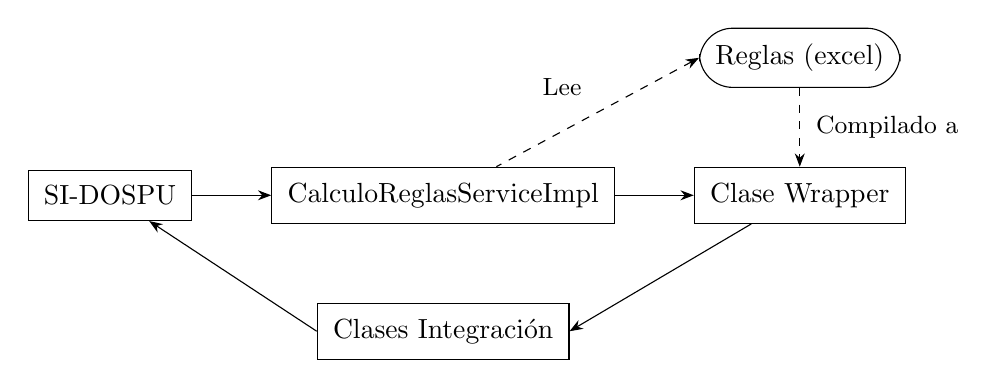
\begin{tikzpicture}[
        auto,
        inner sep=2mm,
        box/.style={draw, rectangle, align=center},
        alt-box/.style={draw, rectangle, align=center, rounded corners=12pt},
        pre/.style={Stealth-},
        post/.style={-Stealth},
        alt-pre/.style={dashed, Stealth-},
        alt-post/.style={dashed, -Stealth},
    ]
        \node[box] (system) {SI-DOSPU};
        \node[box, right=of system] (service) {CalculoReglasServiceImpl}
            edge[pre] (system);
        \node[box, below=of service] (clases) {Clases Integración}
            (clases.west) edge[post] (system);
        \node[box, right=of service] (wrapper)  {Clase Wrapper}
            edge[pre] (service)
            edge[post] (clases.east);
        \node[alt-box, above=of wrapper] (rules)  {Reglas (excel)}
            edge[alt-post] node {\small Compilado a} (wrapper)
            (rules.west) edge[alt-pre] node[swap] {\small Lee} (service);
    \end{tikzpicture}
\end{figure}
\end{frame}
\begin{comment}
En el diagrama se puede ver la estructura resultante de la integración con el sistema. Los rectángulos sin bordes redondeados representan una o varias clases Java, siendo la comunicación entre las mismas por llamado de sus respectivos métodos.

CalculoReglasServiceImpl es la implementación del servicio mencionado anteriormente.

Las clases de integración son las clases utilizadas de forma directa desde las reglas. Estas clases abstraen algunos de los detalles de implementación del sistema, con el fin de reducir la complejidad de las reglas de negocios.
\end{comment}

\subsection{Ejemplo: cálculo de voluntario jubilado}

\begin{frame}{Ejemplo: cálculo de voluntario jubilado}
    \begin{figure}
        \centering
        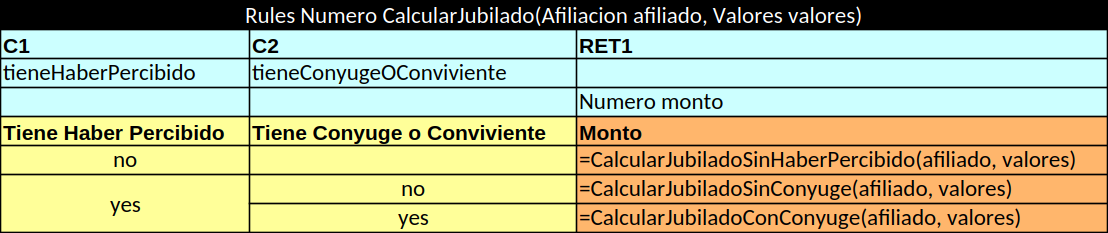
\includegraphics[width=\textwidth]{tables/jubilado.png}
    \end{figure}
    \begin{block}{Inferencia de parámetros}
        \texttt{objeto.getCampo()} \rightarrow \texttt{campo}
    \end{block}
\end{frame}
\begin{comment}
En esta tabla comienza en cálculo de la cuota base, sin los aportes extra, para los voluntarios jubilados.

De forma general, las primeras filas definen las condiciones y acciones o, como en este caso, el retorno de la regla. En particular se define las expresiones que se utilizan para esto y los parámetros que se utilizan dentro de las expresiones. (En la presentación doy un poco más de detalle señalando las celdas en particular)

También podemos ver una de las características de OpenL Tablets, la inferencia de parámetros. Los nombres utilizados dentro de las expresiones pueden hacer referencia a los parámetros definidos para la expresión, los parámetros de la tabla o los campos de estos últimos, adicionalmente, la llamada a un método getter de un objeto de java es equivalente al acceso a un campo. Dado el uso de campos privados en los objetos, este uso no resulta ambiguo.
\end{comment}

\begin{frame}{Ejemplo: cálculo de voluntario jubilado}
    \begin{block}{Dispersión de valores}
        \texttt{Afiliacion} y \texttt{Valores} abstraen el acceso a múltiples clases
    \end{block}
    \begin{block}{Manejo de errores}
        \begin{itemize}
            \item tipo \texttt{Response<T>}
            \item Errores
                \begin{itemize}
                    \item recuperables
                    \item no recuperables
                \end{itemize}
        \end{itemize}
    \end{block}
\end{frame}
\begin{comment}
Las clases Afiliacion y Valores, en la tabla anterior, tienen dos propósitos.

El primero es abstraer el acceso a múltiples clases internas para la obtención de información necesaria para el cálculo, como el haber jubilatorio del afiliado. Afiliacion brinda acceso a la información referida al afiliado y Valores a valores de referencia.


Por otro lado, se utilizan para encapsular el manejo de errores. Dentro del sistema, muchos métodos con los que se obtiene información sobre los afiliados retornan el tipo Response<T> que puede ser un valor o un error. Dentro de estos errores, podemos diferenciar entre dos tipos.
- recuperables: son aquellos que comunican información dentro de un estado válido del sistema. Por ejemplo consultar por el haber jubilatorio de un voluntario jubilado que no tiene uno registrado resultará en el retorno de una error. Como se mencinó anteriormente, este es una caso válido para esta subcategoría.
- no recuperables: por otro lado, si una clase debería siempre tener un sueldo registrado, no tenerlo representa un error en la cargo de datos, con lo cual no puede ser recuperado

En el primer caso, se proveen metodos como los vistos en la tabla anterior, tieneHaberPercibido, para consultar sobre la existencia o no de un valor.

En el otro, se eleva una excepción con el error correspondiente, que luego la implementación del servicio se encarga de transformar nuevamente en un valor de tipo Response<T>

En el otro, se eleva una excepción con el error correspondiente, que luego la implementación del servicio se encarga de transformar nuevamente en un valor de tipo Response<T>
\end{comment}

\begin{frame}{Ejemplo: cálculo de voluntario jubilado}
    \begin{figure}
        \centering
        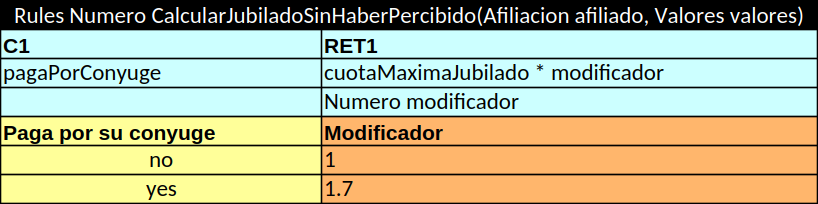
\includegraphics[width=0.7\textwidth]{tables/jubiladoSinHaber.png}
    \end{figure}
\end{frame}
\begin{comment}
En esta tabla se puede apreciar la utilidad de la clase de integración restante Numero. Esta clase actúa como wrapper de la clase BigDecimal, para poder realizar operaciones con los operadores aritméticos y de comparación comunes en lugar de tener que llamar a los métodos correspondiente.    

También se puede utilizar para mantener el detalle del cálculo de la cuota, manteniendo registro de las operaciones llevadas a cabo sobre los valores en lugar de especificar el detalle de forma manual.
\end{comment}

\begin{frame}
    \begin{figure}
        \centering
        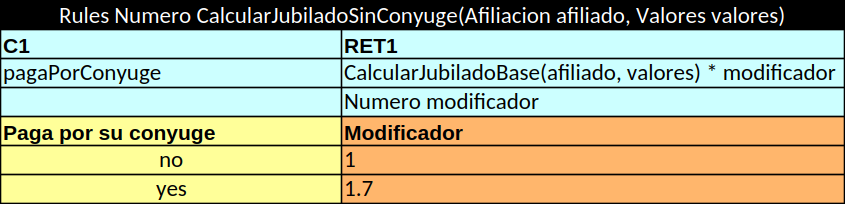
\includegraphics[width=0.75\textwidth]{tables/jubiladoSinConyuge.png}
    \end{figure}
    \begin{figure}
        \centering
        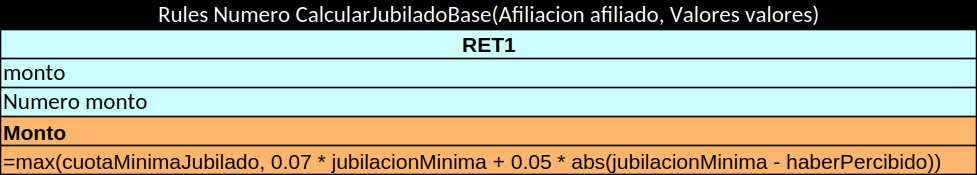
\includegraphics[width=0.9\textwidth]{tables/jubiladoBase.png}
    \end{figure}
\end{frame} 
\begin{comment}
(Explicación breve con base en lo explicado en la parte de afiliaciones)
\end{comment}

\begin{frame}
    \begin{figure}
        \centering
        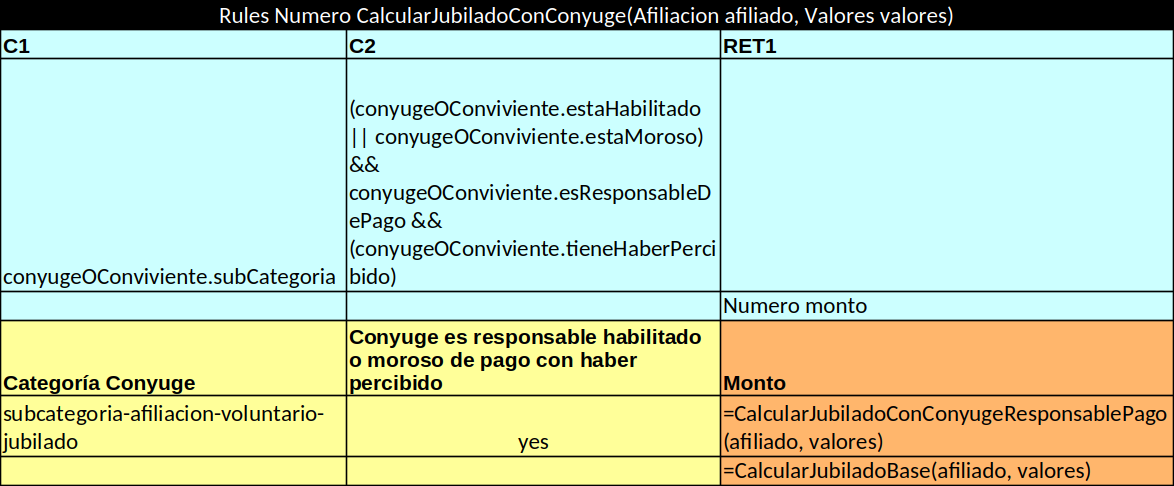
\includegraphics[width=\textwidth]{tables/jubiladoConConyuge.png}
    \end{figure}
    \begin{figure}
        \centering
        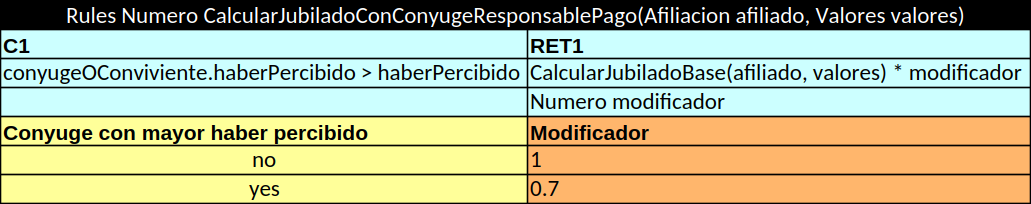
\includegraphics[width=0.9\textwidth]{tables/jubiladoConConyugeResponsable.png}
    \end{figure}
\end{frame}
\begin{comment}
(Explicación breve con base en lo explicado en la parte de afiliaciones)
\end{comment}

% TODO:
\begin{frame}{Ejemplo de un cambio}
    
\end{frame}
\begin{comment}
\end{comment}

\section{Resultados}

% TODO: 
\begin{frame}{Resultados}
    
\end{frame}
\begin{comment}
\end{comment}

\section{Conclusiones}

% TODO: 
\begin{frame}{Conclusiones}
    
\end{frame}
\begin{comment}
\end{comment}

\end{document}
